\section{Durchführung und Aufbau}
\label{sec:Durchführung}

In Abbildung \ref{img:LIV} sieht man den verwendeten modular aufgebauten Lock-In-Verstärker.
\begin{figure}[H]
	\centering
	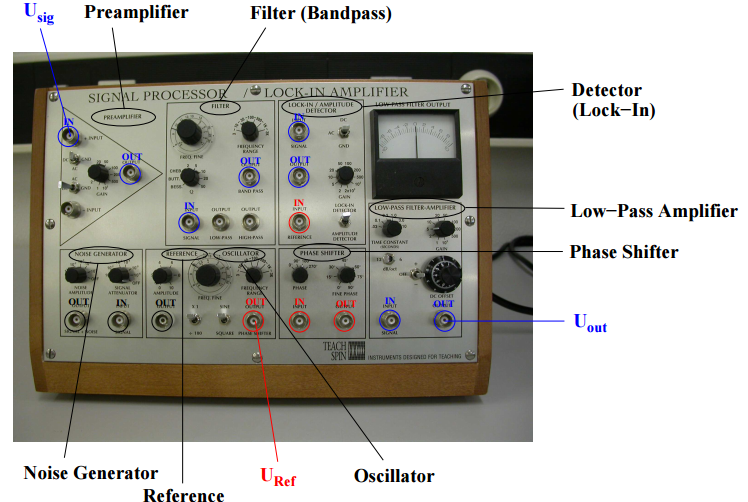
\includegraphics[height=9cm]{picture/LIV.png}
	\caption{Im Versuch verwendeter Lock-In-Verstärker. \cite[3]{sample}}
  \label{img:LIV}
\end{figure}
Im folgenden werden die einzelnen Module kurz erklärt:
\begin{itemize}
	\item Der Vorverstärker verstärkt das eingehende Signal.
	\item Der Filter (Bandpass) filtert höhere und niedrigere Frequenzen aus dem Nutzsignal.
	\item Mit dem Lock-In / Detektor werden die Signal- und die Referenzspannung multipliziert und verstärkt.
	\item Mit dem Phasenverschieber wir die Phasenverschiebung zwischen Signal- und Referenzspannung eingestellt.
	\item Der Rauschgenerator kann ein Rauschen zu dem Nutzsignal hinzufügen.
	\item Der Funktionengenerator erzeugt das Nutz- und das Referenzsignal mit der Frequenz $\omega_0$.
	\item Der Tiefpassfilter / Verstärker gibt $U_\text{out}$ aus und kann dieses noch verstärken.
\end{itemize}
\newpage

\subsection{Schaltung für die Phasenabhängigkeit der Ausgangsspannung}
Als Erstes wird an dem rechten Ausgang des Funktionengenerators der Phasenverschieber angeschlossen, welcher mit dem unteren Eingang des Lock-In verbunden wird. Danach wir der linke Ausgang des Funktionengenerators mit dem Eingang des Rauschgenerators verbunden. Von dem Rauschgenerator wird nun eine Verbindung zum Vorverstärker hergestellt, der Vorverstärker wir nun mit dem Filter verbunden. Von dem Filter(Bandpass) soll eine Verbindung zum Lock-In-Verstärker hergestellt werden. Zuletzt wird von dem Ausgang des Lock-In-Verstärkers zu dem Eingang des Tiefpassfilters und dem Channel 1 des Oszilloskops eine Verbindung hergestellt. Der Aufbau wird schematisch in Abbildung \ref{img:V1} dargestellt.
\begin{figure}[H]
	\centering
	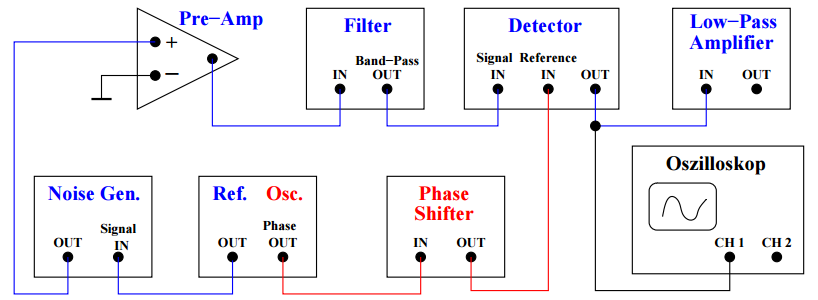
\includegraphics[height=4.2cm]{picture/Aufbau-Versuch1.png}
	\caption{Schaltung für den ersten Versuch. \cite[4]{sample}}
  \label{img:V1}
\end{figure}

\subsection{Photodetektorschaltung}
Für die Photodetektorschaltung wird der Rauschgenerator aus der Schaltung entfernt und durch eine LED mit Photodetektor ersetzt. Die LED wird an den linken Ausgang des Funktionengenerators angeschlossen und der Photodetektor wird mit dem Vorverstärker verbunden. Die LED und der Photodetektor stehen sich auf einem Stab gegenüber. Der Abstand zwischen den beiden Bauteilen kann variiert werden und wird mit einer auf dem Stab angebrachten Millimeterskala gemessen. Der Aufbau wird schematisch in Abbildung \ref{img:V2} dargestellt.
\begin{figure}[H]
	\centering
	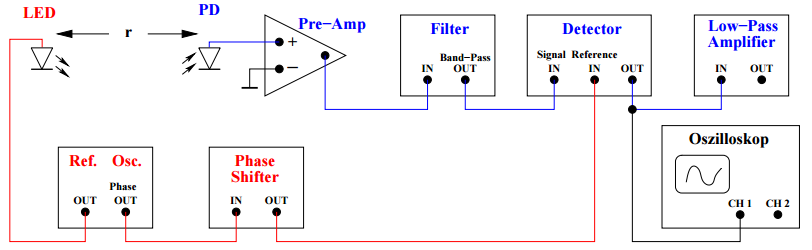
\includegraphics[height=4.2cm]{picture/Photodetektorschaltung.png}
	\caption{Die Photodetektorschaltung. \cite[5]{sample}}
  \label{img:V2}
\end{figure}
